\documentclass[10pt,a4paper]{article}
\usepackage[utf8]{inputenc}
\usepackage[T1]{fontenc}
\usepackage[french]{babel}
\usepackage{listings}
\usepackage{hyperref}
\usepackage{color}
\usepackage{amsmath}
\usepackage{amsfonts}
\usepackage{amssymb}
\usepackage{graphicx}
\usepackage{float}

\definecolor{coolblack}{rgb}{0.10, 0.18, 0.30}

\lstset{belowskip=\baselineskip}
\hypersetup{
	colorlinks=true,
	linkcolor=black,  
	urlcolor=coolblack,
	citecolor=black,
}

\author{
	Jian Chen
	\and
	Valentin Mention
}
\title{SR03\\
	Rapport du Devoir n°1}


\begin{document}
	
	\maketitle
	\newpage
	
	\tableofcontents
	\newpage
	
	\section{Définition du projet}
	\renewcommand{\labelitemi}{-}
	
	\subsection{Contexte}
	Le premier devoir de SR03 consiste en la réalisation d'une application de messagerie entre plusieurs clients et un serveur, afin de créer un espace où plusieurs utilisateurs peuvent communiquer entre eux.
	
	\subsection{Objectifs}
	Nous avons fixés plusieurs exigences auxquelles doit répondre ce projet :
	
	\paragraph{Côté client}
	\begin{itemize}
		\item Le client doit disposer d'une interface console pour envoyer des messages au serveur
		\item L'actualisation des messages doit être automatique et le client doit pouvoir recevoir des messages pendant qu'il est en train lui-même de saisir un message
		\item Si le serveur n'est pas sur le port par défaut, le client doit pouvoir spécifier le port de connexion 
		\item Le client doit pouvoir se déconnecter quand il le souhaite
		\item Chaque utilisateur doit être identifié par un nom d'utilisateur unique
		\item Si possible, les clients auront la possibilité d'échanger par messages privés
	\end{itemize}

	\paragraph{Côté serveur}
	\begin{itemize}
		\item Le serveur doit récupérer les messages envoyés par un utilisateur et les redistribuer à tous les autres utilisateurs
		\item Le serveur doit accepter les connexions entrantes et gérer un certain nombre d'utilisateurs connectés
		\item Le serveur est responsable de la vérification des messages envoyés par l'utilisateur, et de du processus d'assignation de nom à chaque client connecté
		\item Le serveur doit pouvoir recevoir plusieurs messages d'utilisateurs différents simultanément
		\item Le serveur doit être résilient aux erreurs et ne pas planter en cas d'événement inattendu ou d'exceptions. Le nombre d'exceptions non-gérées doit être minime à nul.
	\end{itemize}

	\subsection{Concepts}
	Afin de satisfaire ces objectifs, il est nécessaire de comprendre plusieurs concepts.\par
	
	\subsubsection{Les threads}
	Les threads sont une forme de "sous-processus" qui s'exécutent en parallèle du processus principal, et qui en partagent le même espace mémoire. Ils sont nécessaires dans notre projet du côté client, afin de pouvoir récupérer les entrées utilisateurs, sans bloquer la lecture des messages provenant du serveur. Ils sont également nécessaire au serveur, afin de pouvoir interagir simultanément avec tous les clients connectés. Chaque connexion d'un utilisateur sera donc géré par un thread sur le serveur.
	
	\subsubsection{Les sockets}
	Les sockets sont une interface logicielle qui servent d'interface avec les fonctions réseau d'un système d'exploitation. Chaque socket est responsable d'une connexion avec un périphérique réseau, dans notre cas il s'agit de la connexion client-serveur. Ainsi, le client possède un unique socket qui gère les échanges avec le serveur, et le serveur dispose d'un socket par client.
	
	
	\section{Implémentation en Java}
	
	\subsection{Classes du programme client}
	
	\subsubsection{\href{https://sr03_chen_mention.gitlab.utc.fr/devoir1_doc/client/MessageInput.html}{MessageInput}}
	
	 \href{https://sr03_chen_mention.gitlab.utc.fr/devoir1_doc/client/MessageInput.html}{MessageInput} gère les entrées utilisateurs. Il s'agit d'une tâche bloquante, donc cette classe implémente \href{https://docs.oracle.com/javase/7/docs/api/java/lang/Runnable.html}{Runnable} afin d'être exécutée dans son propre thread et de ne pas bloquer l'exécution de tout le programme. L'implémentation de Runnable est préférée de manière générale à Threads, car plus flexible \cite{runnable:threads}. Lorsque l'utilisateur saisit un message, la méthode bloquante $\href{https://sr03_chen_mention.gitlab.utc.fr/devoir1_doc/client/MessageInput.html#readstr()}{readstr}$ retourne le message saisi, qui est envoyé au serveur par la méthode $\href{https://sr03_chen_mention.gitlab.utc.fr/devoir1_doc/client/MessageInput.html#send(java.lang.String)}{send}$, sauf si le message est "/exit" qui provoque la déconnexion et l'arrêt du client.
	
	\subsubsection{\href{https://sr03_chen_mention.gitlab.utc.fr/devoir1_doc/client/MessageReceptor.html}{MessageReceptor}} 
	\href{https://sr03_chen_mention.gitlab.utc.fr/devoir1_doc/client/MessageReceptor.html}{MessageReceptor} récupère les messages envoyés par le serveur et les affiche dans la console. Il n'y a aucun traitement des données côté client, les données sont affichés telles qu'elles sont reçues et c'est le serveur qui est chargé de la mise en forme.
	
	
	\subsubsection{\href{https://sr03_chen_mention.gitlab.utc.fr/devoir1_doc/client/Client.html}{Client}}
	\href{https://sr03_chen_mention.gitlab.utc.fr/devoir1_doc/client/Client.html}{Client} ne possède qu'une méthode main, qui constitue le point d'entrée du programme. Cette méthode vérifie les arguments qui lui sont passés, établie la connexion avec le serveur et lance les threads de \href{https://sr03_chen_mention.gitlab.utc.fr/devoir1_doc/client/MessageInput.html}{MessageInput} et \href{https://sr03_chen_mention.gitlab.utc.fr/devoir1_doc/client/MessageReceptor.html}{MessageReceptor}.
	
	
	\subsection{Classes du programme serveur}
	
	\subsubsection{\href{https://sr03_chen_mention.gitlab.utc.fr/devoir1/server/Channel.html}{Channel}}
	\href{https://sr03_chen_mention.gitlab.utc.fr/devoir1/server/Channel.html}{Channel} est chargée de l'interaction avec un unique client, depuis le choix de son nom d'utilisateur jusqu'à sa déconnexion. Cette classe implémente \href{https://docs.oracle.com/javase/7/docs/api/java/lang/Runnable.html}{Runnable} et s'exécute dans son propre thread. Elle possède une méthode bloquante $\href{https://sr03_chen_mention.gitlab.utc.fr/devoir1/server/Channel.html#init()}{init}$ appelée dans la méthode $\href{https://sr03_chen_mention.gitlab.utc.fr/devoir1/server/Channel.html#run()}{run}$ au lancement du thread, qui récupère et vérifie le nom d'utilisateur du client. Quand l'utilisateur est correctement authentifié, le canal s'ajoute à la liste de tous les canaux actifs qui est partagée et synchronisée entre toutes les instances de  \href{https://sr03_chen_mention.gitlab.utc.fr/devoir1/server/Channel.html}{Channel}. \par
	
	Une fois que l'utilisateur a été ajouté à la liste, la méthode $\href{https://sr03_chen_mention.gitlab.utc.fr/devoir1/server/Channel.html#run()}{run}$ vérifie en continue si l'utilisateur envoie des messages. Dès qu'un message est reçu, il est analysé afin de déterminer dans un premier temps s'il est valide (c'est à dire non vide) et s'il s'agit d'une commande. Auquel cas la méthode $\href{https://sr03_chen_mention.gitlab.utc.fr/devoir1/server/Channel.html#execCommand(java.lang.String)}{execCommand}$ est appelée pour prendre en compte cette commande. Sinon, on considère qu'il s'agit d'un message pour tous les autres utilisateurs et on appelle $\href{https://sr03_chen_mention.gitlab.utc.fr/devoir1/server/Channel.html#broadcast(server.Message)}{broadcast}$ pour transmettre le message aux autres utilisateurs. \par
	
	La diffusion du message se fait par itération sur la liste de canaux, en appelant la méthode $\href{https://sr03_chen_mention.gitlab.utc.fr/devoir1/server/Channel.html#send(java.lang.String)}{send}$ de chaque canal et en lui passant le message à transmettre. \par
	
	Alternativement, il est possible pour les utilisateurs d'envoyer un message privé à un seul utilisateur. Ce cas est traité par $\href{https://sr03_chen_mention.gitlab.utc.fr/devoir1/server/Channel.html#execCommand(java.lang.String)}{execCommand}$, transmis ensuite à $\href{https://sr03_chen_mention.gitlab.utc.fr/devoir1/server/Channel.html#privateSend(java.lang.String,java.lang.String)}{privateSend}$ qui identifie dans la liste de canaux celui qui échange avec le destinataire du message et appelle sa méthode $\href{https://sr03_chen_mention.gitlab.utc.fr/devoir1/server/Channel.html#send(java.lang.String)}{send}$.
	
	
	
	\subsubsection{\href{https://sr03_chen_mention.gitlab.utc.fr/devoir1/server/Message.html}{Message}}
	\href{https://sr03_chen_mention.gitlab.utc.fr/devoir1/server/Message.html}{Message} est une structure de donnée constituée de deux chaînes de caractères, une pour l'auteur du message et l'autre pour le contenu. Lorsque du texte doit être transmis aux clients, un objet \href{https://sr03_chen_mention.gitlab.utc.fr/devoir1/server/Message.html}{Message} est transmis à tous les \href{https://sr03_chen_mention.gitlab.utc.fr/devoir1/server/Channel.html}{Channel}, qui l'enverront à leur client respectif, sauf s'il s'agit du client à l'origine du message.
	
	\subsubsection{\href{https://sr03_chen_mention.gitlab.utc.fr/devoir1/server/Message.html}{Serveur}}
	\href{https://sr03_chen_mention.gitlab.utc.fr/devoir1/server/Message.html}{Serveur} contient la méthode main et est le point d'entrée du programme serveur. Il accepte dans une boucle infinie toutes les connexions des utilisateurs et leur assigne un \href{https://sr03_chen_mention.gitlab.utc.fr/devoir1/server/Channel.html}{Channel}. Il est possible de lui passer en paramètre le port sur lequel ouvrir la connexion.
	

	
	\section{Déploiement}
	
	\subsection{Cloner le dépôt Git}
	
	Afin de déployer ce projet, il faut récupérer les fichiers sources disponibles sur Gitlab. Pour cela, le moyen préféré est de "cloner" le dépôt, bien qu'il soit également possible de télécharger le projet dans une archive.\\
	
	La commande à utiliser pour cloner le projet est :
	\begin{verbatim}
	git clone git@gitlab.utc.fr:sr03_chen_mention/devoir1.git devoir1
	\end{verbatim}
	 Ce dépôt étant privé, il est nécessaire d'utiliser un compte autorisé à y accéder. De plus, git doit être correctement configuré pour utiliser le compte en question ou une clé SSH associée.
	 
	 Il est recommandé de toujours utiliser la dernière version disponible de la branche master. 
	
	\subsection{Compiler l'application}
	
	Afin de lancer les applications clients et serveur, il est nécessaire de les compiler. En ouvrant le projet avec un IDE, cela peut être réalisé automatiquement. Sinon, il est possible d'effectuer la compilation manuellement.
	
	Pour compiler manuellement, se placer dans le répertoire racine du projet (c'est à dire le dossier "devoir1") et ouvrir un invite de commande. Les instructions ci-dessous sont peuvent être réalisés automatiquement en exécutant le fichier $build.sh$ disponible à la racine du projet.
	
	\color{red}Attention ! \color{black} L'environnement de compilation doit disposer du JDK Java 8 au minimum et la version 13 est recommandée.
	
	\subsubsection{Compilation du serveur}
	\begin{verbatim}
	> mkdir .binaries
	> javac -d ./.binaries ./src/server/*.java
	> cd ./.binaries
	> jar cvmf ../src/server/META-INF/MANIFEST.MF Server.jar server
	> cd ../
	\end{verbatim}
	
	\subsubsection{Compilation du client}
	\begin{verbatim}
	> mkdir .binaries
	> javac -d ./.binaries ./src/client/*.java
	> cd ./.binaries
	> jar cvmf ../src/client/META-INF/MANIFEST.MF Client.jar client
	\end{verbatim}
	
	Si la compilation aboutit, il est à présent possible dans le dossier $.binaries$ d'exécuter les fichiers $Client.jar$ et $Server.jar$.
	
	\subsection{Démarrer l'application} \label{sub:execution}
	
	Pour lancer l'exécution du client ou du serveur, définir le répertoire actif d'un invite de travail sur $.binaries$ ou tout autre dossier contenant les fichiers exécutables. Bien qu'il soit possible d'exécuter l'application avec les fichiers .class également générés, nous ne traiterons pas ce cas ici.
	
	Il est nécessaire de démarrer le serveur avant le client. Il faut un invite de commande par programme lancé.
	
	\paragraph{Pour lancer le serveur}
	\begin{verbatim}
		> java -jar Server.jar
	\end{verbatim}
	
	\paragraph{Pour lancer le serveur en spécifiant le port}
	\begin{verbatim}
		> java -jar Server.jar 1234
	\end{verbatim}
	
	\paragraph{Pour lancer le client}
	\begin{verbatim}
	> java -jar Client.jar
	\end{verbatim}
	
	\paragraph{Pour lancer le client en spécifiant l'IP du serveur}
	\begin{verbatim}
	> java -jar Client.jar 192.168.0.1
	\end{verbatim}
	
	\paragraph{Pour lancer le client en spécifiant l'IP et le port du serveur} 
	
	\begin{verbatim}
	> java -jar Client.jar 192.168.0.1 1234
	\end{verbatim}
	
	Attention, pour le client on ne peut pas spécifier le port sans spécifier l'IP
	
	\subsection{Exemple de fonctionnement}
	
	\subsubsection{Instructions}
	
	Pour démontrer les fonctionnalités de notre application il est nécessaire d'avoir au moins 3 invites de commandes lancés, 4 étant préférables afin de pouvoir constater le fonctionnement des messages privés. Il est également préférable d'utiliser des consoles de type Bash, qui supportent les caractères accentués (non supporté par Windows, ce qui cause des problèmes d'affichage).
	
	En suivant les instructions données en \ref{sub:execution}, lancer une instance serveur et trois instances clients sans passer de paramètres (les paramètres par défaut sont utilisés). Si demandé par le système d'exploitation, autoriser l'application à accéder au réseau.
	
	Constater la bonne connexion des clients au serveur, puis entrer un nom d'utilisateur pour le premier client. Pour le second client, essayer de saisir le même nom que précédemment (sensible à la casse, mais pas aux espaces, qui sont supprimés), et constater le refus du serveur. Dans la console serveur, on pourra remarquer que seules les connexions et déconnexions des sockets sont indiquées, sans préciser si l'utilisateur est identifié ou pas. Il s'agit d'un choix de conception.
	
	Saisir un nom valide pour les deux clients restants, et vérifier dans l'invite du premier client l'annonce de la connexion des deux autres. Envoyer un message depuis un client : le message est transmis aux deux autres avec le pseudonyme de celui l'ayant envoyé.
	
	Tester à présent les commandes, en tapant /help pour en afficher la liste. On note que la commande n'est pas transmise aux autres utilisateurs. Tenter d'envoyer un message privé à un autre utilisateur, en utilisant :
	\begin{verbatim}
	> /Bob Bonjour Bob !
	\end{verbatim}
	
	S'il existe un utilisateur nommé Bob (encore une fois, la casse est importante), on observe dans son invite de commande (et on remarque que le troisième client ne voit rien de cet échange) :
	
	\begin{verbatim}
	> >> Alice: Bonjour Bob !
	\end{verbatim}
	
	Les messages privés sont reconnaissables aux doubles carets $>>$ les précédents. S'il n'existe pas d'utilisateur nommé Bob, Alice verra marqué dans son invite :
	
	\begin{verbatim}
	> Commande ou utilisateur inconnu ! /help pour la liste des commandes
	\end{verbatim}
	
	\subsubsection{Démonstration}
	
	\begin{figure}[H]
	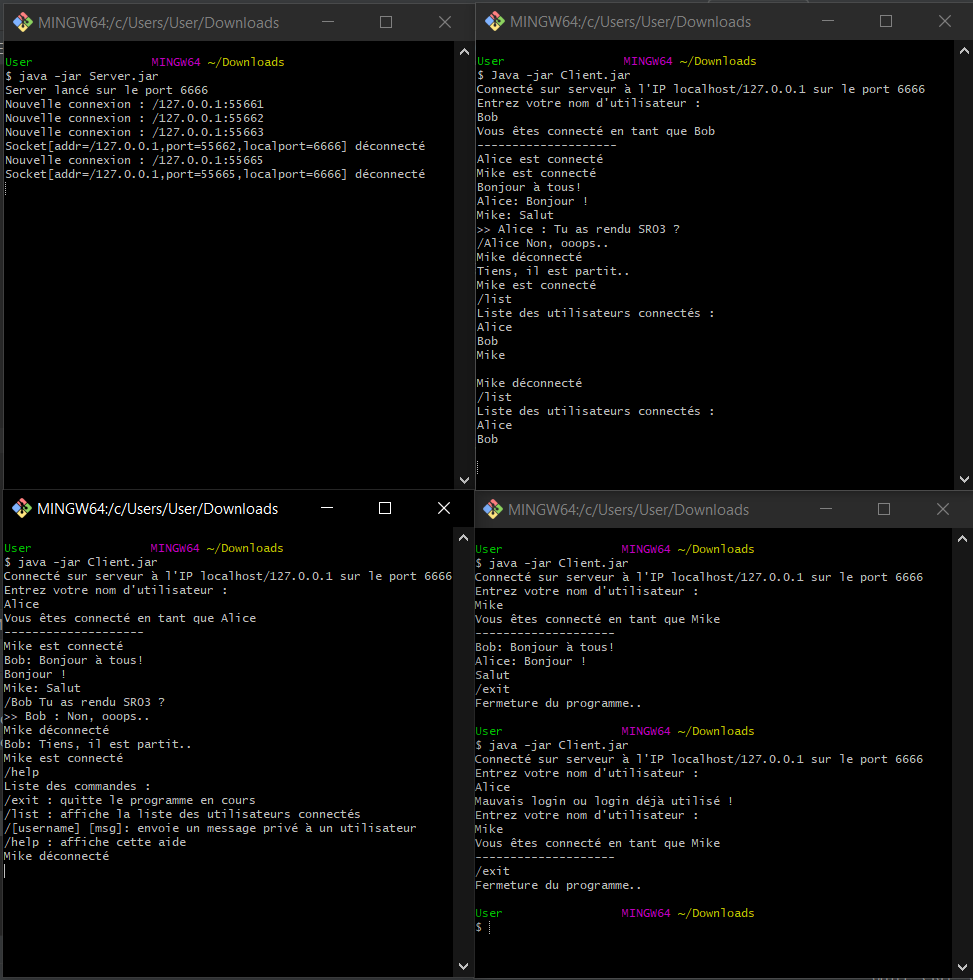
\includegraphics[width=\linewidth]{ressources/demo.png}
	\caption{Exemple de fonctionnement avec un serveur et trois clients}
	\end{figure}
	
	
	\section{Schémas de fonctionnement simplifié}
	
	\subsection{Client}
	
	\begin{figure}[H]
		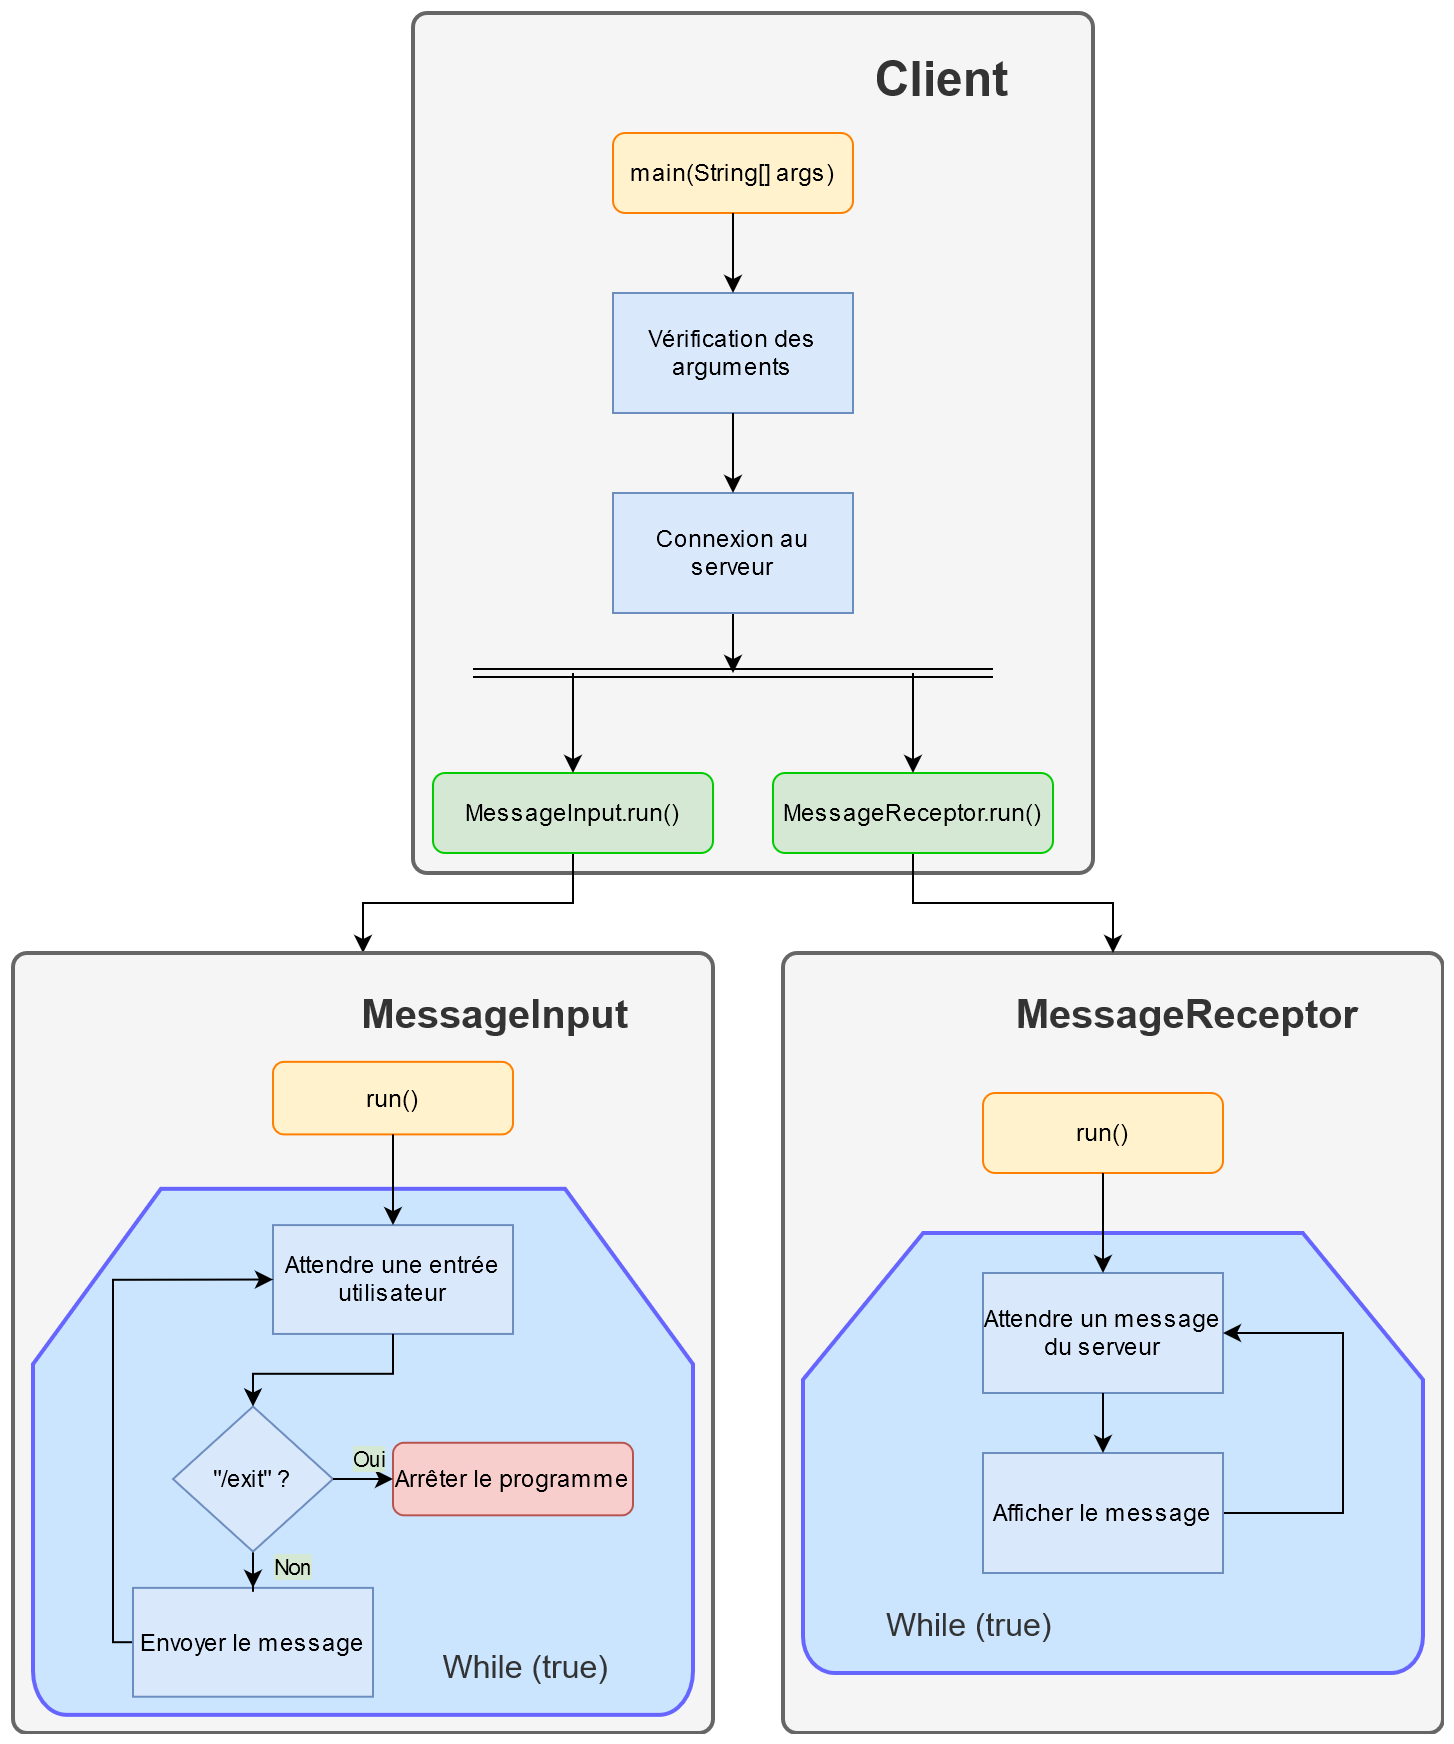
\includegraphics[width=\linewidth]{ressources/client_package.png}
	\end{figure}
	
	\subsection{Serveur}
	
	\begin{figure}[H]
		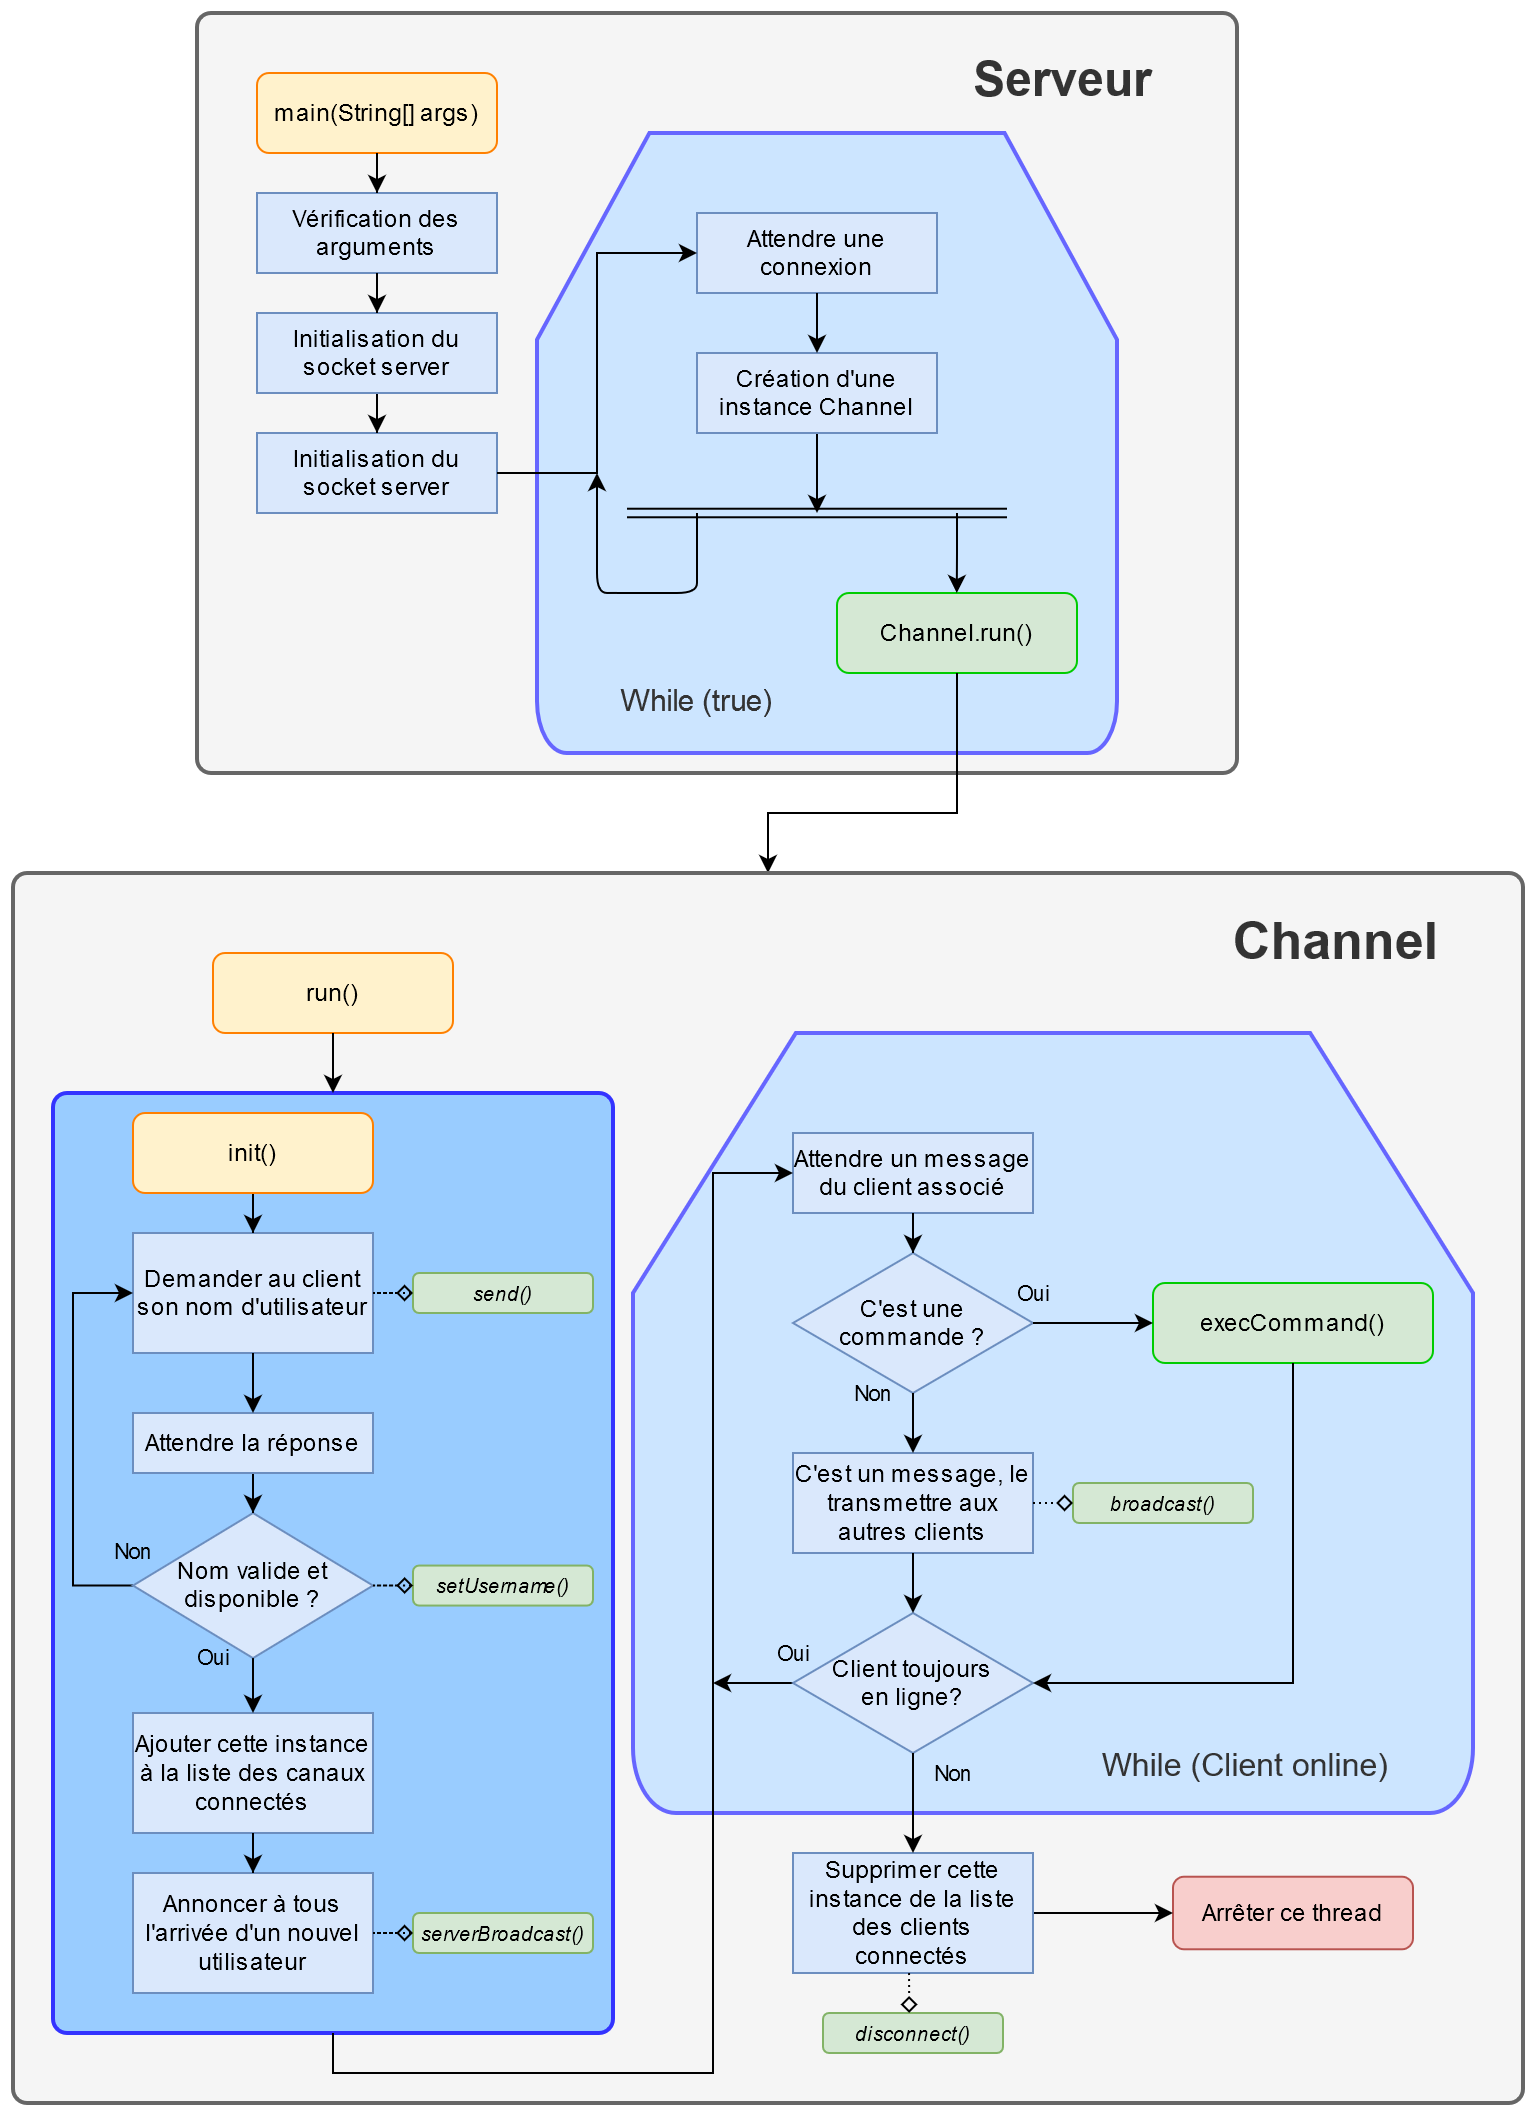
\includegraphics[width=\linewidth]{ressources/server_package.png}
	\end{figure}
	
	
	
	\newpage
	
	
	
	\newpage
	
	\appendix
	\section{Liens importants}
	
	Javadoc du projet : \url{https://sr03_chen_mention.gitlab.utc.fr/devoir1/index.html}
	
	Page des releases :
	\url{https://gitlab.utc.fr/sr03_chen_mention/devoir1/-/releases}
	
	Racine du dépôt git :
	\url{https://gitlab.utc.fr/sr03_chen_mention/devoir1/-/tree/master}
	
	
	\begin{thebibliography}{5}
		\bibitem{runnable:threads} \url{https://stackoverflow.com/questions/541487/implements-runnable-vs-extends-thread-in-java}
	\end{thebibliography}
	
	
	
\end{document}